\documentclass[twoside,11pt]{jmlr}

% The JMLR class loads natbib, hyperref, graphicx, amsmath and amssymb.
% Do not reload natbib: JMLR uses author-year plainnat citations.
\usepackage{mathtools}
\usepackage{bm}
\usepackage{booktabs}
\usepackage{enumitem}
\usepackage{array}
\usepackage{multirow}
\usepackage{tikz}
\usetikzlibrary{arrows.meta,positioning,fit,shapes.geometric}
\graphicspath{{figures/}}

\hypersetup{
    colorlinks=true,
    linkcolor=blue!60!black,
    citecolor=blue!60!black,
    urlcolor=blue!60!black
}

\numberwithin{equation}{section}

\newcommand{\KL}{\operatorname{KL}}
\newcommand{\E}{\mathbb{E}}
\newcommand{\R}{\mathbb{R}}
\newcommand{\dd}{\mathrm{d}}
\newcommand{\Law}{\mathcal{L}}
\newcommand{\Path}{\mathcal{X}}
\newcommand{\pdata}{\pi_{\mathrm{data}}}
\newcommand{\pbase}{\pi_0}
\newcommand{\ptarget}{\pi_1}
\newcommand{\diver}{\nabla\!\cdot}
\newcommand{\scrR}{\mathsf{R}}
\newcommand{\scrP}{\mathsf{P}}
\newcommand{\scrQ}{\mathsf{Q}}
\newcommand{\bb}{\bm b}
\newcommand{\vv}{\bm v}
\newcommand{\xx}{\bm x}
\newcommand{\zz}{\bm z}
\newcommand{\yy}{\bm y}
\newcommand{\uu}{\bm u}
\newcommand{\eps}{\varepsilon}
\newcommand{\F}{\bm F}
\newcommand{\J}{\bm J}
\newcommand{\Var}{\operatorname{Var}}
\newcommand{\Tr}{\operatorname{Tr}}
\newcommand{\Id}{\operatorname{Id}}
\newcommand{\supp}{\operatorname{supp}}

\jmlrvolume{0}
\jmlryear{2026}
\jmlrpages{1--\pageref{jmlrend}}
\firstpageno{1}

\title[Path-Space Variational Bridges]{Path-Space Variational Bridges:\
Couplings, Gauges, and Field-Line Bridges for Generative Modeling}

\author[Zhang]{%
\Name{Tiantian Zhang} \Email{t.zhang8@columbia.edu}\\
\addr Department of Computer Science\\
Columbia University, New York, NY 10027, USA
}

\editor{}

\begin{document}
\maketitle

\begin{abstract}
Diffusion models, score-based stochastic differential equations, flow matching, rectified flows, Schr\"odinger bridges, and Poisson-flow generative models are often presented as separate generative paradigms. This paper proposes a common mathematical object behind them: a \emph{path-space variational bridge}. The construction has four ingredients: an endpoint coupling, a conditional bridge law on latent paths, a Markovian projection that turns non-causal bridges into causal generative dynamics, and a probability-current gauge that decides whether the same marginal path is represented as an ODE, an SDE, or an augmented-space field flow. Beyond this organizational view, we introduce two concrete tools. First, we define the \emph{Markovization gap}, the irreducible loss incurred when a bridge path posterior is compressed into a causal Markov vector field; this gives a bridge-selection diagnostic and a caustic criterion for deterministic bridges. Second, we formalize Poisson and electrostatic generative models as \emph{field-line bridge kernels}: the endpoint coupling is induced by hitting maps of an augmented potential field, and the bridge measure is a Dirac or small-noise Doob bridge along field lines. A small two-dimensional experiment illustrates that changing only the endpoint coupling can reduce the estimated Markovization gap by two orders of magnitude. The goal is not to replace existing stochastic-interpolant or diffusion-bridge theories, but to make explicit the graphical-model, bridge-geometry, and gauge degrees of freedom that they partially share.
\end{abstract}

\begin{keywords}
diffusion models, rectified flows, stochastic interpolants, path-space variational inference, bridge matching, Poisson flows, field matching
\end{keywords}

\paragraph{Status.}
This is a preliminary framework paper. The theory and toy diagnostic are intended to sharpen the mathematical proposal; the manuscript still needs larger empirical validation before being positioned as a full benchmark paper.

\section{Introduction}

Many recent generative models learn a continuous transformation from a simple distribution to a data distribution. Diffusion probabilistic models learn to reverse a noising Markov chain and are trained through a variational bound \citep{sohldickstein2015nonequilibrium,ho2020ddpm,kingma2021vdm}. Score-based SDE models describe the same idea in continuous time and derive both reverse-time SDE samplers and equivalent probability-flow ODEs \citep{song2021score}. Flow matching and rectified flow learn an ODE vector field by regressing conditional velocities of prescribed probability paths \citep{lipman2023flow,liu2022rectified,tong2024cfm}. Stochastic interpolants explicitly unify deterministic flows and stochastic diffusions through interpolating processes and probability currents \citep{albergo2023flows,albergo2023stochastic}. Schr\"odinger bridge methods replace deterministic transport by entropy-regularized stochastic transport \citep{tong2024sf2m,shi2023dsbm}. Poisson-flow and electrostatic field-matching models take a different-looking route: data distributions become charges or capacitor plates in an augmented space, and generation follows field lines \citep{xu2022pfgm,xu2023pfgmpp,kolesov2025field,manukhov2025ifm,shlenskii2026duality}.

The working hypothesis of this paper is that the common structure is not a particular SDE, ODE, score, velocity, noise schedule, or electric field. The common structure is a \emph{latent path graphical model}. A modeler first specifies how a simple endpoint and a data endpoint are coupled. Then the modeler specifies a conditional path law, or bridge, between those endpoints. This produces a teacher path measure. The learned generator is a causal Markov process obtained by projecting that teacher path measure onto a Markov family. Finally, the same marginal evolution can be represented by different stochastic gauges: a deterministic probability-flow ODE, a noisy SDE with a score correction, or an augmented-space field flow.

This perspective leads to a more precise slogan:
\begin{center}
\emph{Diffusion and rectified flow are not fundamentally different graphical models; they are different bridge and gauge choices inside a path-space latent-variable model.}
\end{center}

\subsection{Contributions}

\begin{enumerate}[leftmargin=2em]
    \item We define a \emph{path-space variational bridge} using an endpoint coupling, a conditional bridge kernel, and a learned Markov decoder process.
    \item We introduce the \emph{Markovization gap}, an irreducible conditional-variance objective that measures how difficult it is to compress a bridge into a causal Markov dynamics. This turns the usual projection identity into a bridge-selection diagnostic.
    \item We state a probability-current gauge theorem: if a marginal density path solves a continuity equation, then an infinite family of SDEs with different diffusion matrices realizes the same marginals by changing the drift with a score/divergence correction.
    \item We formalize Poisson, electrostatic, and interaction-field generative models as field-line bridge kernels in augmented space, including deterministic hitting-map bridges and small-noise Doob bridge regularizations.
    \item We report a small synthetic diagnostic showing that changing only the endpoint coupling, from independent pairing to minibatch OT pairing, sharply lowers the Markovization gap of a straight-line bridge.
\end{enumerate}

\section{Relation to existing unifications}
\label{sec:positioning}

The closest existing frameworks already capture large parts of the story. Stochastic interpolants construct processes between two prescribed distributions and show that the same interpolant density satisfies transport and Fokker--Planck equations with tunable diffusion coefficients \citep{albergo2023stochastic}. Diffusion Flow Matching describes a bridge construction using a coupling plus a deterministic or stochastic bridge and studies KL guarantees for Brownian bridges \citep{silveri2024dfm}. Unified bridge algorithms relate flow matching, OT flow matching, Schr\"odinger bridge flow matching, and DSBM \citep{kim2025unified}. Latent stochastic interpolants move the interpolant into a jointly learned encoder--decoder latent model using a continuous-time ELBO \citep{singh2025lsi}. Field-matching work connects electrostatic or interaction fields to conditional flow matching and shows that forward-only IFM can be bijectively related to CFM, while more general IFM can be more expressive \citep{shlenskii2026duality}.

The present framework differs in emphasis rather than by denying these unifications. It treats the endpoint coupling, bridge law, Markov projection, and stochastic gauge as four separate graphical-model primitives. This separation matters for at least three reasons. First, it makes the coupling an inference object, allowing the VAE-like case $\Gamma_\phi(\dd z,\dd x)=q_\phi(\dd z\mid x)\pdata(\dd x)$. Second, it treats field-line models as bridge kernels rather than as exceptions to flow-based modeling. Third, it provides a diagnostic, the Markovization gap, for deciding whether a bridge geometry is easy or hard to compress into a Markov decoder.

\begin{table}[t]
\centering
\small
\begin{tabular}{@{}p{0.22\linewidth}p{0.28\linewidth}p{0.39\linewidth}@{}}
\toprule
Framework & Main primitive & What the present paper adds \\
\midrule
Stochastic interpolants & Interpolating process and probability current & Explicit endpoint inference coupling, path-space VAE view, and field-line bridge kernels. \\
Diffusion Flow Matching & Coupling plus deterministic/stochastic bridge; Markovian projection & General graphical-model decomposition, gauge as independent choice, and non-Brownian field bridges. \\
Latent stochastic interpolants & Learned encoder/decoder plus latent SI ELBO & Treats the bridge kernel and stochastic gauge as separately learnable or selectable objects. \\
PFGM / EFM / IFM & Augmented electrostatic or interaction field & Formalizes fields as hitting-map bridge kernels and defines the caustic/Markovization gap. \\
\bottomrule
\end{tabular}
\caption{Positioning relative to active unification directions.}
\label{tab:related_positioning}
\end{table}

\begin{figure}[t]
\centering
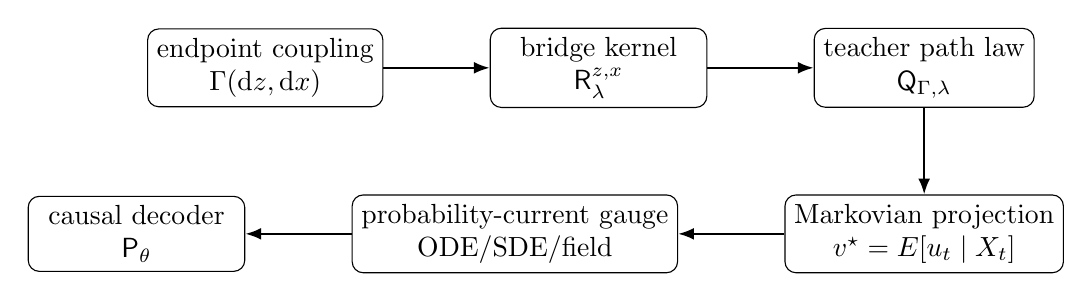
\begin{tikzpicture}[
    node distance=1.10cm and 1.35cm,
    box/.style={draw, rounded corners, align=center, minimum height=0.9cm, minimum width=2.75cm},
    arrow/.style={-{Latex[length=2mm]}, thick}
]
    \node[box] (coupling) {endpoint coupling\\$\Gamma(\dd z,\dd x)$};
    \node[box, right=of coupling] (bridge) {bridge kernel\\$\mathsf R^{z,x}_\lambda$};
    \node[box, right=of bridge] (teacher) {teacher path law\\$\mathsf Q_{\Gamma,\lambda}$};
    \node[box, below=of teacher] (projection) {Markovian projection\\$v^\star=\E[u_t\mid X_t]$};
    \node[box, left=of projection] (gauge) {probability-current gauge\\ODE/SDE/field};
    \node[box, left=of gauge] (decoder) {causal decoder\\$\mathsf P_\theta$};
    \draw[arrow] (coupling) -- (bridge);
    \draw[arrow] (bridge) -- (teacher);
    \draw[arrow] (teacher) -- (projection);
    \draw[arrow] (projection) -- (gauge);
    \draw[arrow] (gauge) -- (decoder);
\end{tikzpicture}
\caption{Path-space variational bridge: choose endpoint coupling and bridge geometry, aggregate a teacher path measure, project it to a causal Markov process, then choose a stochastic gauge for the same probability current.}
\label{fig:psvb}
\end{figure}

\section{Path-space variational bridge}

Let $\mathcal M$ be the state space, usually $\R^d$ or an augmented space such as $\R^d\times\R^D$. Let $\Path=C([0,1],\mathcal M)$ be path space. Let $X_t:\Path\to\mathcal M$ denote the coordinate process. Let $\pbase$ be a simple base distribution and let $\ptarget=\pdata$ be the data distribution.

\begin{definition}[Endpoint coupling]
An endpoint coupling is a probability measure
\begin{equation}
    \Gamma(\dd z,\dd x)\in \Pi(\pbase,\ptarget),
\end{equation}
where $\Pi(\pbase,\ptarget)$ is the set of couplings whose first marginal is $\pbase$ and second marginal is $\ptarget$.
\end{definition}

Examples include independent coupling, minibatch optimal-transport coupling, entropic optimal-transport coupling, paired data coupling, or a learned encoder coupling
\begin{equation}
    \Gamma_\phi(\dd z,\dd x)=q_\phi(\dd z\mid x)\pdata(\dd x).
\end{equation}
The last case is the most VAE-like: the base endpoint is not merely noise but an inferred latent variable.

\begin{definition}[Conditional bridge kernel]
For each endpoint pair $(z,x)$, a bridge kernel is a path-space probability measure
\begin{equation}
    \scrR^{z,x}_\lambda(\dd X_{0:1}),
    \qquad X_0=z,\quad X_1=x,
\end{equation}
where $\lambda$ denotes bridge hyperparameters or learnable bridge parameters.
\end{definition}

The bridge kernel is where geometry enters. It may be deterministic, Brownian, Schr\"odinger, Hamiltonian, harmonic, electrostatic, or learned. Given $\Gamma$ and $\scrR_\lambda$, define the aggregated teacher path law
\begin{equation}
    \scrQ_{\Gamma,\lambda}(\dd X_{0:1})
    =\int \scrR^{z,x}_\lambda(\dd X_{0:1})\,\Gamma(\dd z,\dd x).
    \label{eq:teacher_path_law}
\end{equation}

\begin{definition}[Path-space variational bridge]
A path-space variational bridge consists of
\begin{equation}
    (\Gamma_\phi,\scrR_\lambda,\scrP_\theta,p_\psi),
\end{equation}
where $\Gamma_\phi$ is an endpoint inference coupling, $\scrR_\lambda$ is a conditional bridge, $\scrP_\theta$ is a causal Markov path law initialized from $\pbase$, and $p_\psi(x\mid y_1)$ is an optional observation decoder.
\end{definition}

The simplest generative model uses $Y_1$ itself as the sample. A more VAE-like model decodes from $Y_1$ through $p_\psi(x\mid Y_1)$. The continuous-time ELBO has the formal form
\begin{equation}
    \log p_{\theta,\psi}(x)
    \ge
    \E_{\scrQ_\phi(\dd Y_{0:1}\mid x)}
    \left[
        \log p_\psi(x\mid Y_1)
        -\log\frac{\dd \scrQ_\phi(\cdot\mid x)}{\dd \scrP_\theta}(Y_{0:1})
    \right],
    \label{eq:path_elbo}
\end{equation}
whenever the conditional inference path law is absolutely continuous with respect to the generative path law. If both laws share a diffusion covariance and differ only in drift, Girsanov's theorem turns the path KL term into an integrated drift-matching cost. This is the continuous-time analog of a hierarchical VAE with infinitely many latent layers.

\section{Markovian projection and the Markovization gap}
\label{sec:markovization}

Assume first that $\scrQ=\scrQ_{\Gamma,\lambda}$ is supported on differentiable paths, or more generally that it has a local velocity or drift target $u_t$ satisfying
\begin{equation}
    \frac{\dd}{\dd t} f(X_t)=\nabla f(X_t)\cdot u_t
\end{equation}
for smooth test functions in the deterministic case. We want a causal Markov ODE
\begin{equation}
    \dd Y_t=v_\theta(Y_t,t)\,\dd t,\qquad Y_0\sim\pbase,
    \label{eq:ode_decoder}
\end{equation}
that has the same one-time marginals as the teacher, or at least approximates them.

\begin{definition}[Markovization gap]
For a teacher path law $\scrQ$ with local target $u_t$, define the Markovization gap
\begin{equation}
    \mathfrak G(\scrQ)
    =\inf_v\int_0^1 \E_{\scrQ}\left[\|u_t-v(X_t,t)\|^2\right]\dd t.
    \label{eq:markov_gap_def}
\end{equation}
This quantity depends on the coupling and bridge, not on neural-network approximation error.
\end{definition}

\begin{proposition}[Projection identity and irreducible bridge loss]
For a fixed teacher path law $\scrQ$, the population minimizer of
\begin{equation}
    \mathcal L_{\mathrm{FM}}(v)
    =\int_0^1 \E_{\scrQ}\left[\|u_t-v(X_t,t)\|^2\right] \dd t
    \label{eq:fm_loss}
\end{equation}
is
\begin{equation}
    v^\star(x,t)=\E_{\scrQ}\left[u_t\mid X_t=x\right].
    \label{eq:markov_projection_velocity}
\end{equation}
Moreover,
\begin{equation}
    \mathfrak G(\scrQ)
    =\int_0^1\E_{\scrQ}\left[\Tr\,\Var(u_t\mid X_t)\right]\dd t.
    \label{eq:markov_gap_variance}
\end{equation}
\end{proposition}

Thus, flow matching is a Markovian projection of a non-causal bridge. The non-causal bridge may know both endpoints $(Z,X)$; the learned generator can only look at the current state and time. Equation~\eqref{eq:markov_gap_variance} gives a bridge-selection diagnostic: low gap means that the bridge is nearly Markov when observed only through $X_t$; high gap means that many hidden endpoint configurations induce conflicting local velocities at the same location and time.

For an It\^o teacher process
\begin{equation}
    \dd X_t=\beta_t\,\dd t+\sigma_t\,\dd B_t,
\end{equation}
with possibly non-Markov adapted drift $\beta_t$, the Markovian projected drift is similarly
\begin{equation}
    b^\star(x,t)=\E_{\scrQ}[\beta_t\mid X_t=x],
    \label{eq:markov_projection_drift}
\end{equation}
under standard mimicking assumptions. Diffusion flow matching with Brownian bridges can be read in precisely this way \citep{silveri2024dfm}.

\section{Probability-current gauge}
\label{sec:gauge}

The central object is the marginal density path $\rho_t$ and its probability current $\J_t$. If an ODE velocity $v_t$ transports $\rho_t$, then
\begin{equation}
    \partial_t\rho_t+\nabla\cdot(\rho_t v_t)=0,
    \qquad \J_t=\rho_t v_t.
    \label{eq:continuity}
\end{equation}
For an SDE
\begin{equation}
    \dd X_t=b_t(X_t)\,\dd t+\sigma_t(X_t)\,\dd B_t,
    \qquad a_t=\sigma_t\sigma_t^\top,
    \label{eq:sde}
\end{equation}
the Fokker--Planck equation can be written as a continuity equation
\begin{equation}
    \partial_t\rho_t+\nabla\cdot \J_t=0,
    \qquad
    J_{t,i}=\rho_t b_{t,i}-\frac12\sum_j\partial_j(a_{t,ij}\rho_t).
    \label{eq:prob_current}
\end{equation}

\begin{theorem}[Probability-current gauge]
Suppose $\rho_t$ and $v_t$ solve Eq.~\eqref{eq:continuity}. Let $a_t(x)\succeq 0$ be a smooth diffusion matrix. Define
\begin{equation}
    b_i^{(a)}(x,t)
    =v_i(x,t)+\frac{1}{2\rho_t(x)}\sum_j\partial_j\left(a_{ij}(x,t)\rho_t(x)\right).
    \label{eq:gauge_drift}
\end{equation}
Then the SDE with drift $b^{(a)}$ and diffusion matrix $a$ has the same marginal density path $\rho_t$ as the ODE velocity $v_t$, provided the Fokker--Planck equation is well posed. If $a_t(x)=g(t)^2 I$, then
\begin{equation}
    b^{(a)}(x,t)=v_t(x)+\frac{g(t)^2}{2}\nabla\log\rho_t(x).
    \label{eq:scalar_gauge}
\end{equation}
\end{theorem}

This theorem separates \emph{transport} from \emph{gauge}. The marginal path is determined by $\J_t=\rho_t v_t$. A deterministic flow uses $a=0$. A diffusion uses $a\neq0$ and compensates with a score term. Thus the score is not an independent ontology; it is the correction needed to express the same probability current in a noisy gauge.

\section{Field-line bridge kernels for Poisson and electrostatic flows}
\label{sec:field_bridges}

The least standard part of the framework is the claim that Poisson and electrostatic methods are bridge geometries. This section makes the bridge kernel explicit.

Let $\Omega\subset\R^m$ be an augmented state space with two transverse boundary hypersurfaces $S_0$ and $S_1$. In PFGM-like settings, $S_1$ is the data hyperplane $\R^d\times\{0\}$ and $S_0$ is a large sphere or source surface in the augmented space. In EFM-like settings, $S_0$ and $S_1$ can be source and target capacitor plates. Let $\Phi:\Omega\to\R$ be a potential and
\begin{equation}
    \F(y)=-\nabla\Phi(y)
\end{equation}
be the induced field. For PFGM, $\Phi$ is a Green-function potential whose distributional Laplacian equals a charge measure supported on the data hyperplane; for EFM, $\Phi$ solves a capacitor-like electrostatic problem with source and target charges \citep{xu2022pfgm,kolesov2025field}. Assume that $\F$ is smooth and non-vanishing away from the charged boundary and that its flow is transverse to $S_0$ and $S_1$.

Let $\varphi_s(z)$ denote the solution of
\begin{equation}
    \frac{\dd}{\dd s}\varphi_s(z)=\F(\varphi_s(z)),
    \qquad \varphi_0(z)=z.
    \label{eq:field_flow}
\end{equation}
Let
\begin{equation}
    \tau(z)=\inf\{s>0:\varphi_s(z)\in S_1\}
\end{equation}
be the hitting time and define the hitting map
\begin{equation}
    T_\Phi(z)=\varphi_{\tau(z)}(z).
    \label{eq:hitting_map}
\end{equation}
Choose any smooth increasing clock $r_z:[0,1]\to[0,\tau(z)]$ with $r_z(0)=0$ and $r_z(1)=\tau(z)$, and define the normalized field line
\begin{equation}
    \gamma_z(t)=\varphi_{r_z(t)}(z),
    \qquad
    u_t(z)=\partial_t\gamma_z(t)=r'_z(t)\F(\gamma_z(t)).
    \label{eq:normalized_field_line}
\end{equation}

\begin{definition}[Deterministic field-line bridge]
Given a source measure $\mu_0$ on $S_0$, the field-induced endpoint coupling is
\begin{equation}
    \Gamma_\Phi=(\Id,T_\Phi)_\#\mu_0.
    \label{eq:field_coupling}
\end{equation}
For $(z,x)$ in the support of $\Gamma_\Phi$, the deterministic field-line bridge kernel is
\begin{equation}
    \scrR^{z,x}_{\Phi}(\dd X_{0:1})
    =\delta_{\gamma_z}(\dd X_{0:1}),
    \qquad x=T_\Phi(z).
    \label{eq:field_line_bridge_kernel}
\end{equation}
The aggregated teacher path law is $\scrQ_\Phi=\int \delta_{\gamma_z}\,\mu_0(\dd z)$.
\end{definition}

This is the promised bridge kernel. It is not a Brownian bridge in data space; it is a deterministic bridge induced by the hitting geometry of a potential field in augmented space. PFGM corresponds to the special case where $\mu_0$ is an asymptotically uniform distribution on a large hemisphere and the potential is generated by data charges on the $z=0$ hyperplane \citep{xu2022pfgm}. PFGM++ varies the dimension of the augmented coordinates and recovers PFGM at $D=1$ and diffusion behavior as $D\to\infty$ \citep{xu2023pfgmpp}.

\begin{definition}[Small-noise field bridge]
For endpoint pairs not exactly generated by the deterministic hitting map, or to obtain an absolutely continuous path measure, define a field-driven diffusion
\begin{equation}
    \dd Y_s=\F(Y_s)\,\dd s+\sqrt{2\epsilon}\,\dd B_s.
    \label{eq:field_diffusion}
\end{equation}
The $\epsilon$-regularized field bridge is the Doob bridge
\begin{equation}
    \scrR^{z,x}_{\Phi,\epsilon}
    =\Law\left(Y_{0:1}\mid Y_0=z,\,Y_1=x\right),
    \label{eq:doob_field_bridge}
\end{equation}
a field-biased analog of a Brownian bridge. As $\epsilon\to0$, it concentrates on field lines when a unique field-line connection exists.
\end{definition}

The next result connects field-line bridges to Markov projection and explains what information is lost when the field-line path law is compressed into a Markov velocity.

\begin{theorem}[Field-line bridges and caustic Markovization gap]
Let $\scrQ_\Phi$ be the deterministic field-line bridge law defined by Eq.~\eqref{eq:field_line_bridge_kernel}, and let $X_t=\gamma_Z(t)$ for $Z\sim\mu_0$. Assume the maps are smooth and all expectations below are finite. Then:
\begin{enumerate}[leftmargin=2em]
    \item The marginals $\rho_t=(\gamma_t)_\#\mu_0$ solve the weak continuity equation
    \begin{equation}
        \partial_t\rho_t+\nabla\cdot \J_t=0,
        \qquad
        \J_t=(\gamma_t)_\#(u_t\mu_0).
    \end{equation}
    \item The Markovian velocity
    \begin{equation}
        v^\star(y,t)=\E[u_t(Z)\mid \gamma_Z(t)=y]
    \end{equation}
    realizes the same one-time marginal path, in the sense that $\J_t=\rho_t v^\star(\cdot,t)$ whenever $\rho_t$ admits a density.
    \item The irreducible field-to-flow compression loss is
    \begin{equation}
        \mathfrak C_\Phi
        =\int_0^1\E\left[\Tr\,\Var(u_t(Z)\mid \gamma_Z(t))\right]\dd t.
        \label{eq:field_caustic_gap}
    \end{equation}
    It is zero if and only if the field-line velocity $u_t(Z)$ is a measurable function of the current point $\gamma_Z(t)$ for almost every $t$. In particular, it is zero when $\gamma_t$ is injective $\mu_0$-a.s.; it is positive when different field lines pass through the same point-time with different velocities.
\end{enumerate}
\end{theorem}

We call Eq.~\eqref{eq:field_caustic_gap} a \emph{caustic gap}. It does not say that nonzero gap prevents matching one-time marginals: the projected velocity still transports the marginal density. Rather, it quantifies the path information discarded by the causal Markov representation. This is precisely where an augmented field description can be useful even when an equivalent probability path exists.

\section{Instantiations}

\begin{table}[t]
\centering
\small
\begin{tabular}{@{}p{0.18\linewidth}p{0.30\linewidth}p{0.20\linewidth}p{0.22\linewidth}@{}}
\toprule
Model family & Coupling/bridge choice & Learned object & Gauge/view \\
\midrule
DDPM / score SDE & fixed Gaussian noising bridge from data to noise & score or denoiser & stochastic gauge, variational path ELBO \\
Flow matching & conditional probability path between endpoints & velocity field & ODE gauge \\
Rectified flow & straight-line bridge $X_t=(1-t)Z+tX$ & $\E[X-Z\mid X_t]$ & deterministic bridge and ODE gauge \\
Brownian bridge / DFM & Brownian bridge conditioned on endpoints & Markovian projected drift & stochastic bridge, SDE gauge \\
Schr\"odinger bridge & KL-optimal path measure relative to Brownian reference & forward/backward drifts or scores & entropy-regularized stochastic transport \\
PFGM / EFM / IFM & hitting-map field-line bridge in augmented space & field lines or interaction field & augmented-space field gauge \\
\bottomrule
\end{tabular}
\caption{Several generative paradigms as choices inside the same path-space bridge template.}
\label{tab:instances}
\end{table}

\subsection{Diffusion models as path-space VAEs}

A discrete DDPM defines a fixed inference/noising process
\begin{equation}
    q(x_{1:T}\mid x_0)=\prod_{t=1}^T q(x_t\mid x_{t-1})
\end{equation}
and a learned reverse Markov chain
\begin{equation}
    p_\theta(x_{0:T})=p(x_T)\prod_{t=1}^T p_\theta(x_{t-1}\mid x_t).
\end{equation}
The latent variables are the entire chain $(x_1,\ldots,x_T)$. The training bound is a variational bound on $\log p_\theta(x_0)$ \citep{ho2020ddpm,kingma2021vdm}. In the path-space bridge language, the inference bridge starts at data and ends at a tractable base distribution; the decoder reverses this path. The graphical model is therefore a hierarchical VAE with a fixed, very deep encoder.

In continuous time, the score-based SDE formulation chooses a forward noising SDE and uses the time-reversal formula to define a generative reverse SDE whose drift depends on $\nabla\log\rho_t$ \citep{song2021score}. The probability-flow ODE is the zero-noise representation of the same marginal path.

\subsection{Rectified flow and flow matching}

For straight-line rectified flow, sample $(Z,X)\sim\Gamma$ and define
\begin{equation}
    X_t=(1-t)Z+tX,
    \qquad u_t=X-Z.
\end{equation}
The projection loss becomes
\begin{equation}
    \mathcal L_{\mathrm{RF}}(v_\theta)
    =\E_{t,Z,X}\left[\|X-Z-v_\theta((1-t)Z+tX,t)\|^2\right].
    \label{eq:rf_loss}
\end{equation}
The learned ODE velocity is the causal projection
\begin{equation}
    v^\star(x,t)=\E[X-Z\mid (1-t)Z+tX=x].
\end{equation}
Thus, rectified flow is not essentially about straight lines; it is about projecting a chosen non-causal bridge into a causal Markov flow. Straightness is a bridge prior.

General flow matching replaces the deterministic line with a family of conditional probability paths $p_t(\cdot\mid z,x)$ and conditional vector fields. It still minimizes a regression loss whose population minimizer is the marginal vector field \citep{lipman2023flow,tong2024cfm}.

\subsection{Brownian bridges and Schr\"odinger bridges}

A Brownian bridge from $z$ to $x$ with variance parameter $\epsilon$ can be written informally as
\begin{equation}
    X_t=(1-t)z+t x+\sqrt{\epsilon}\,(B_t-tB_1).
    \label{eq:brownian_bridge}
\end{equation}
Aggregating Eq.~\eqref{eq:brownian_bridge} over a coupling $\Gamma$ yields a path law whose Markovian projection gives a diffusion model. Diffusion flow matching analyzes precisely such bridge-induced path measures and the KL error of their learned projections \citep{silveri2024dfm}.

Schr\"odinger bridges go one step further: instead of fixing the Brownian bridge kernel, they search for the path measure closest in KL to a Brownian reference among all path measures with prescribed endpoints. This makes the bridge geometry adaptive but entropy-regularized. Recent matching algorithms seek scalable approximations to these bridges \citep{tong2024sf2m,shi2023dsbm,kim2025unified}.

\subsection{Gaussian bridge: score, noise, denoiser, and velocity are reparameterizations}

Consider the Gaussian conditional path
\begin{equation}
    X_t=\alpha_t X+\sigma_t\eps,
    \qquad \eps\sim\mathcal N(0,I),
    \label{eq:gaussian_path}
\end{equation}
where $X\sim\pdata$. Let $\rho_t$ be the density of $X_t$ and $s_t(x)=\nabla\log\rho_t(x)$. By Tweedie-style conditioning,
\begin{equation}
    \E[\eps\mid X_t=x]=-\sigma_t s_t(x).
    \label{eq:noise_score}
\end{equation}
The velocity target is
\begin{align}
    v^\star(x,t)
    &=\E[\dot \alpha_t X+\dot\sigma_t\eps\mid X_t=x]\\
    &=\frac{\dot\alpha_t}{\alpha_t}x+
    \left(\frac{\dot\alpha_t\sigma_t^2}{\alpha_t}-\dot\sigma_t\sigma_t\right)s_t(x).
    \label{eq:velocity_score_relation}
\end{align}
Hence denoising, noise prediction, score prediction, and velocity prediction are linear reparameterizations once the bridge schedule $(\alpha_t,\sigma_t)$ is fixed. This explains why diffusion and Gaussian flow matching are often interchangeable at the level of learned information, even if their samplers and parameterizations differ.

\section{A toy diagnostic: coupling changes Markovization difficulty}
\label{sec:toy}

The framework suggests a simple diagnostic: estimate $\mathfrak G(\scrQ)$ before training a neural generator. We sampled $n=1000$ points from a two-dimensional standard normal base and an eight-Gaussian target. We used the same straight-line bridge in both conditions. The only change was the endpoint coupling: independent random pairing versus a minibatch OT assignment minimizing squared Euclidean cost. For each time $t$, we estimated $\E\Tr\Var(X-Z\mid X_t)$ by replacing the conditional mean velocity with a $32$-nearest-neighbor estimate in $X_t$-space.

\begin{figure}[t]
\centering

\includegraphics[width=0.92\linewidth]{toy_projection_gap.pdf}
\caption{Toy Markovization-gap diagnostic. The bridge family is fixed to the straight line $X_t=(1-t)Z+tX$. Changing only the endpoint coupling from independent pairing to minibatch OT reduces the estimated integrated Markovization gap from $4.935$ to $0.038$. This is not a benchmark claim; it illustrates that the framework yields an actionable pre-training diagnostic for coupling and bridge choices.}
\label{fig:toy_gap}
\end{figure}

This experiment is deliberately small. Its purpose is to show that the decomposition is operational rather than purely taxonomic: endpoint coupling affects how much hidden endpoint information must be discarded by the Markov projection. Larger experiments should test whether low Markovization gap correlates with faster training, lower curvature, fewer solver steps, or better sample quality.

\section{Training objectives suggested by the framework}

The framework separates four learning choices.

\paragraph{1. Learn or choose the endpoint coupling.}
A simple choice is independent coupling $\pbase\otimes\pdata$. A transport-biased choice uses minibatch OT or entropic OT. A VAE-like choice learns $q_\phi(z\mid x)$ and induces $\Gamma_\phi(\dd z,\dd x)=q_\phi(\dd z\mid x)\pdata(\dd x)$. The coupling controls semantic alignment and path complexity.

\paragraph{2. Learn or choose the bridge.}
A deterministic bridge gives flow matching. A Brownian bridge gives diffusion flow matching. A Schr\"odinger bridge optimizes the bridge under entropy regularization. A field-line bridge chooses augmented potential geometry. A learnable bridge would optimize $\lambda$ jointly with the generator, analogous to learning the encoder family in a VAE.

\paragraph{3. Project the bridge onto a causal Markov decoder.}
Given samples from the bridge and a local target $u_t$ or $\beta_t$, train
\begin{equation}
    \min_\theta\int_0^1\E\left[\|u_t-v_\theta(X_t,t)\|^2\right]\dd t
\end{equation}
for an ODE gauge, or
\begin{equation}
    \min_\theta\int_0^1\E\left[\|\sigma_t^{-1}(\beta_t-b_\theta(X_t,t))\|^2\right]\dd t
\end{equation}
for a shared-covariance SDE gauge.

\paragraph{4. Choose a gauge for sampling.}
Once a marginal path and current are learned, choose whether to sample with an ODE, with an SDE, or with an augmented-space field. This choice may trade off likelihood tractability, mode coverage, numerical stability, robustness, and guidance behavior.

\section{Open problems}

\paragraph{Learnable bridge posteriors.}
Can we parameterize $\scrR^{z,x}_\lambda$ richly enough to improve sample quality and likelihood while keeping bridge sampling and target computation tractable?

\paragraph{Gauge selection.}
Given a learned current $\J_t$, how should one choose the diffusion matrix $a_t$ for best numerical stability, guidance performance, or likelihood? PFGM++ suggests that intermediate gauges between pure Poisson flow and diffusion can be beneficial \citep{xu2023pfgmpp}.

\paragraph{Path-space amortization.}
A VAE-style model should amortize not only endpoint latent variables but also path variables. Latent Stochastic Interpolants are a concrete step in this direction \citep{singh2025lsi}. More general amortized bridges could connect representation learning with flow/diffusion training.

\paragraph{Field/flow equivalence.}
Recent flow/field matching duality results raise a natural question: which augmented-field geometries are merely reparameterized conditional probability paths, and which are genuinely more expressive \citep{shlenskii2026duality}? The caustic gap in Eq.~\eqref{eq:field_caustic_gap} is one candidate diagnostic for this boundary.

\paragraph{Beyond Brownian reference processes.}
Brownian bridges are mathematically convenient, but not necessarily the best bridge for data with memory, hierarchy, or manifold constraints. Fractional, kinetic, Hamiltonian, or learned reference processes may provide better path priors.

\section{Conclusion}

This manuscript proposes a path-space variational bridge as a unifying mathematical object for diffusion models, rectified flows, flow matching, Brownian/Schr\"odinger bridges, and Poisson/electrostatic flows. The framework has four separable ingredients: endpoint coupling, bridge path measure, Markovian projection, and probability-current gauge. The revised contribution is not only a notation: it provides a bridge-selection quantity, the Markovization gap, and a formal field-line bridge construction for Poisson/electrostatic methods. Under this lens, diffusion models are path-space VAEs with noisy encoder bridges; rectified flows are deterministic bridge projections; Brownian and Schr\"odinger bridges are entropic stochastic bridge choices; and Poisson flows are hitting-map field-line bridges in augmented space.

\appendix

\section{Proofs}

\subsection{Projection identity and Markovization gap}

For any measurable vector field $v$, expand Eq.~\eqref{eq:fm_loss} pointwise in $(x,t)$ using the conditional law of $u_t$ given $X_t=x$:
\begin{align}
    \E[\|u_t-v(X_t,t)\|^2]
    &=\E\left[\E[\|u_t-v(X_t,t)\|^2\mid X_t]\right]\\
    &=\E\left[\Tr\Var(u_t\mid X_t)+\|\E[u_t\mid X_t]-v(X_t,t)\|^2\right].
\end{align}
The variance term is independent of $v$. The unique $L^2$ minimizer is therefore $v^\star(x,t)=\E[u_t\mid X_t=x]$, and integrating over $t$ gives Eq.~\eqref{eq:markov_gap_variance}.

\subsection{Probability-current gauge}

The Fokker--Planck equation for Eq.~\eqref{eq:sde} is
\begin{equation}
    \partial_t\rho_t
    =-\sum_i\partial_i(b_i\rho_t)
    +\frac12\sum_{i,j}\partial_i\partial_j(a_{ij}\rho_t).
\end{equation}
Define
\begin{equation}
    J_i=\rho_t b_i-\frac12\sum_j\partial_j(a_{ij}\rho_t).
\end{equation}
Then $\partial_t\rho_t+\nabla\cdot \J=0$. If $b=b^{(a)}$ as in Eq.~\eqref{eq:gauge_drift}, then
\begin{equation}
    J_i=\rho_t v_i+\frac12\sum_j\partial_j(a_{ij}\rho_t)-\frac12\sum_j\partial_j(a_{ij}\rho_t)=\rho_t v_i.
\end{equation}
Thus the SDE and ODE share the same probability current and hence the same marginal density path, under uniqueness of the Fokker--Planck solution.

\subsection{Field-line bridge theorem}

Let $\rho_t=(\gamma_t)_\#\mu_0$. For any smooth compactly supported test function $f$,
\begin{align}
    \frac{\dd}{\dd t}\int f(y)\rho_t(\dd y)
    &=\frac{\dd}{\dd t}\int f(\gamma_z(t))\mu_0(\dd z)\\
    &=\int \nabla f(\gamma_z(t))\cdot u_t(z)\mu_0(\dd z)\\
    &=\int \nabla f(y)\cdot \J_t(\dd y),
\end{align}
where $\J_t=(\gamma_t)_\#(u_t\mu_0)$ is the vector-valued pushforward measure. This is the weak form of $\partial_t\rho_t+\nabla\cdot \J_t=0$. Disintegrating $\mu_0$ with respect to $\gamma_t$ gives $\J_t=\rho_t v^\star$ with $v^\star(y,t)=\E[u_t(Z)\mid \gamma_Z(t)=y]$. The expression for the caustic gap follows from the projection identity in Appendix~A.1.

\section{Toy experiment details}

The target distribution is an equally weighted mixture of eight Gaussians with centers on a circle of radius $3$ and component standard deviation $0.25$. The base distribution is $\mathcal N(0,I_2)$. The OT coupling is a finite-sample assignment minimizing squared Euclidean cost. The Markovization gap is estimated at $19$ equally spaced times in $[0.05,0.95]$ using a $32$-nearest-neighbor conditional mean estimator for $U=X-Z$ given $X_t=(1-t)Z+tX$. The integrated values in Figure~\ref{fig:toy_gap} are trapezoidal integrals over the time grid. The script used to generate the figure is included in the source package.

\bibliography{references}

\end{document}
